\section{Soution methods}

\subsection{Value Function Iteration}

As a benchmark solution, I solve the problem by using value function iteration. However modifications to the algorithm presented in section \ref{sec:dynamic_programming}. First and foremost, i consider the Q-function instead of the value function, allowing to store state-action value pairs. Second it should be noted that in this formulation multiple of the features are continuous, not allowing for tabular solutions. Thirdly, the dimension of the state-space + the size of the grid made in infeasable\footnote{In my initial attempt to solve the model by value function iteration, i attempted to get the expectation of the value function using Gauss-Hermite integration, and discretizing the statespace. The solution time was infeasible, which was why my approach changed.}
) to solve the model by classical ways of solving a model using backwards induction an discreetizing the state space. 

The solution approach is using backwards induction. Again this makes sense since, we know that the model terminates in a deterministic fashion when the agents reaches a certain age. For each step a large random sample of states is drawn conditional on a given age. For each of these state the agent takes each of the possible actions storing the results. This way a large sample of rewards and states can be generated. Further more for each action taken the the Q-function can be evaluated in the new state new state, Q-function can be evaluated, taken the max of each possible action, allowing for the representation of the value function. A graphical representation of the concept:



The idea is to approximate the integral by using a statistical method, and in this case Deep Learning (another machine learning method would be equally good). Still implore a backwards induction. Consider $f$ to be a machine learning function, that maps from State Space into $\vert \actionspace \vert$. I.e. For a given point in state space a prediction of the value function is computed for each possible action. This implies the method only is feasible for discrete state space. By trying to reduce the mean squared error between the the true values of the Q-function, and the prediction, the $\E[Q(a, s)]$ can be found, which corresponds to integration as could be done using f.x. Gauss Hermite or Monte Carlo integration.

\begin{algorithm}[H]
\SetAlgoLined
\KwResult{Write here the result }
 Initialize $\tilde{Age} = Age_{max}$\;
 Initialize empty lists for storing results: $X, Y$\;
 Initialize memory counter $j=1$\;
 \While{$\tilde{Age} > Age_{min}$}{
  Draw $\{s_i\}_{i=1}^{i=N}$, where $s_i \sim \statespace \mid Age=\tilde{Age}$ \;
  \ForEach{$s_i$}{
  Create empty array $Z$ of length $\mid \actionspace \mid$\;
  \eIf{$\tilde{Age}= Age_{max}$}{
   \ForEach{$a_k \in \actionspace$}{
    $Z[k] \leftarrow r(s_i, a_k)$ \;
   }
   }{
   \ForEach{$a_k \in \actionspace$}{
    $Z[k] \leftarrow r(s_i, a_k)$ + $\gamma \underset{a' \in \actionspace}{\max}\lsp \hat{q}(a', s_i') \rsp$\;
    }
  }
  $Y[j] \leftarrow Z, X[j] \leftarrow s_i$\;
  $j = j + 1$\;
  }
  Estimate $\hat{Q}$ by training a Deep NN using samples from $X, Y$.
 }
 \caption{Deep Q-function iteration solution method}
 \end{algorithm}

Since i use a deep neural network to approximate the $Q$-function, certain things need to be considered. First and foremost I need to consider the architecture of the network. Next I need to consider the train

For each age i draw 20.000 random samples. This is because any smaller number of draw seemed to be detrimental to the performance. This is inline with standard Deep Learning practices. These kinds of network is known to be very data hungry. When training the network i draw a random sample of 100.000 observations. If I have not yet accumulated 100.000 observations the algorithm draws all observations. The architecture of network is fairly simple being a two-layer fully connected network. First layer being 16 nodes wide, second fully connected layer being 8 nodes wide. I found that mini batching, did not seem to work well on this particular task, and instead i train on all observations, using a validation split of 30 \%, training for a maximum of 150 epochs and finally i allow for early stopping, that is, when the validation loss is not furthering decreasing i stop the training of the network. I do allow the algorithm a patience of 5. Implying that the algorithm will try to lower it's validation loss for five additional epochs before terminating the training.


\begin{figure}[ht]
\begin{subfigure}{.5\textwidth}
  \centering
  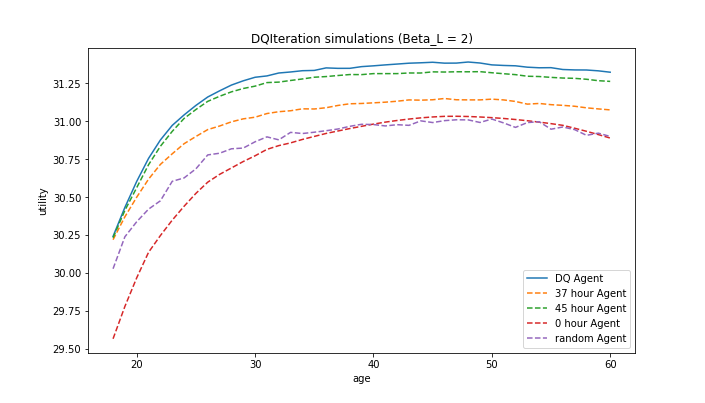
\includegraphics[width=1\linewidth]{figures/dqi_model1_beta_2_solution_benchmark_paths.png}
  \caption{Simulated Paths}
  \label{fig:dqi_solution_beta2_path}
\end{subfigure}%
\begin{subfigure}{.5\textwidth}
  \centering
  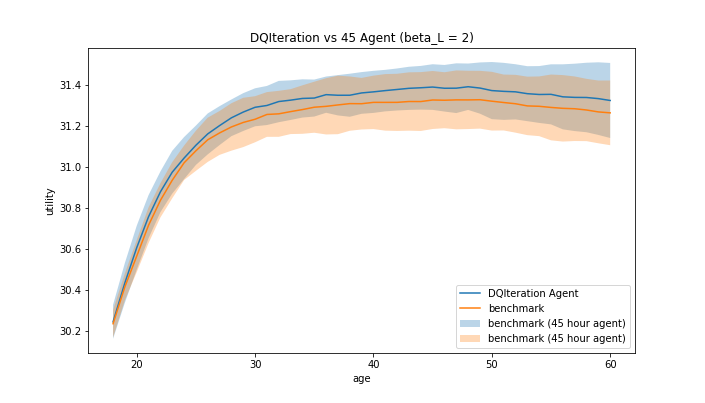
\includegraphics[width=1\linewidth]{figures/dqi_model1_beta_2_solution_benchmark_variance.png}
  \caption{Variance of Paths}
  \label{fig:dqi_solution_beta2_var}
\end{subfigure}
    \caption{Deep Q-iteration solution vs. benchmark $(\beta_L = 2)$}
    \label{fig:dqi_solution_beta2}
\end{figure}

\begin{figure}[ht]
\begin{subfigure}{.5\textwidth}
  \centering
  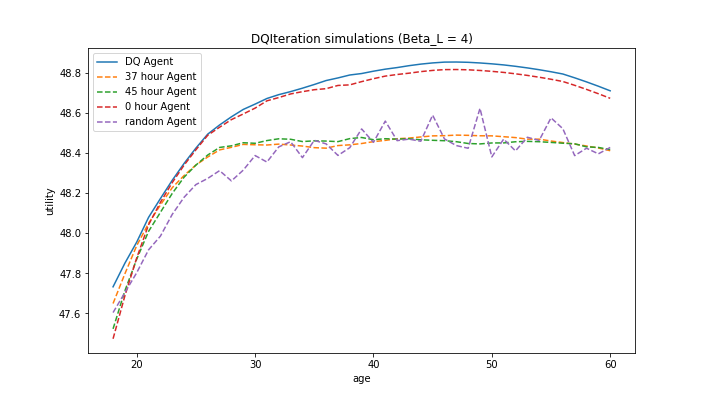
\includegraphics[width=1\linewidth]{figures/dqi_model1_beta_4_solution_benchmark_paths.png}
  \caption{Simulated Paths}
  \label{fig:dqi_solution_beta4_path}
\end{subfigure}%
\begin{subfigure}{.5\textwidth}
  \centering
  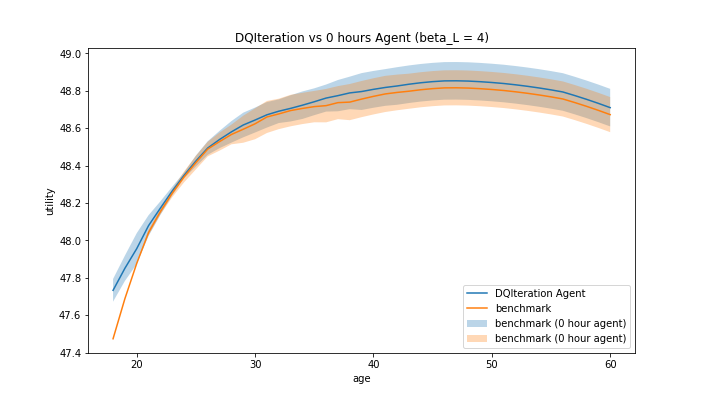
\includegraphics[width=1\linewidth]{figures/dqi_model1_beta_4_solution_benchmark_variance.png}
  \caption{Variance of simulations}
  \label{fig:dqi_solution_beta4_var}
\end{subfigure}
    \caption{Deep Q-iteration solution vs. benchmark $(\beta_L = 4)$}
    \label{fig:dqi_solution_beta4}
\end{figure}

\subsection{Policy Gradient}

\subsection{Q-learning}

\subsection{Double Q-learning}


